\documentclass[11pt]{article}
\usepackage{color}
\usepackage{graphicx}
\usepackage{amsmath,amsthm,amssymb,multirow,paralist}
\usepackage[margin=0.8in]{geometry}
\usepackage[]{algorithm2e}
\usepackage{hyperref}
\usepackage{tikz,forest}
\usetikzlibrary{arrows.meta}

\providecommand{\abs}[1]{\left\vert#1\right\vert}
\providecommand{\norm}[1]{\left\Vert#1\right\Vert}

\begin{document}

\begin{center}
    {\Large \textbf{COM S 474/574: Introduction to Machine Learning}\\Homework \#4}\\

    \linethickness{1mm}\line(1,0){498}

    \begin{enumerate}
        \item Please put required code files and report into a
              compressed file ``HW\#\_FirstName\_LastName.zip''
        \item Unlimited number of submissions are
              allowed on Canvas and the latest one will be graded.
        \item {\color{red} No later submission is accepted.}
        \item Please read and follow submission instructions. No exception
              will be made to accommodate incorrectly submitted files/reports.
        \item All students are required to typeset their reports using
              latex. Overleaf
              (\url{https://www.overleaf.com/learn/latex/Tutorials}) can be a
              good start.
    \end{enumerate}

    \linethickness{1mm}\line(1,0){498}

\end{center}

%%%%%%%%%%%%%%%%%%%%%%%%%%%%%%%%%%%%%%%%%%%%%%%%%%%%%%%%%%%%%%%%%%%%%%%%%%%%%%%

%%%%%%%%%%%%%%%%%%%%%%%%%%%%%%%%%%%%%%%%%%%%%%%%%%%%%%%%%%%%%%%%%%%%%%%%%%%%%%%


\begin{enumerate}

    \item (20 points) \textbf{Hierarchical clustering}

    Use the similarity matrix in Table~\ref{tb:exp1} to perform
    (1) single (MIN) and (2) complete (MAX) link hierarchical
    clustering. Show each step with dendrogram and the
    corresponding similarity matrix update. The dendrogram should
    clearly show the order in which the points are merged.
    Suppose we choose to use 3 clusters, Show the cut in each
    final dendrogram.

    \begin{table}[ht]\label{tb:exp1}
        \centering
        \caption{Similarity matrix.}

        \begin{tabular}{ l| c | c | c | c | c}\hline
                   & \textbf{p1} & \textbf{p2} & \textbf{p3} & \textbf{p4} & \textbf{p5} \\ \hline
            \bf p1 & 1.00        & 0.10        & 0.41        & 0.55        & 0.35        \\
            \bf p2 & 0.10        & 1.00        & 0.64        & 0.47        & 0.98        \\
            \bf p3 & 0.41        & 0.64        & 1.00        & 0.44        & 0.85        \\
            \bf p4 & 0.55        & 0.47        & 0.44        & 1.00        & 0.76        \\
            \bf p5 & 0.35        & 0.98        & 0.85        & 0.76        & 1.00        \\
            \hline
        \end{tabular}
        % \vspace{-5pt}
    \end{table}

    \item (20 points) \textbf{K-Medians Clustering}
    
        The K-means algorithm can be summarized as below:
        \begin{enumerate}
            \item Select K points as the initial centroids.
            \item \textbf{repeat}
            \item \;\;\;\; Form K clusters by assigning all points to the closest centroid.
            \item \;\;\;\; Recompute the centroid of each cluster.
            \item \textbf{until} The centroids don't change.
        \end{enumerate}

        K-medians clustering is a variation of k-means clustering
        where it calculates the median for each cluster to determine
        its center instead of using the mean. Also, K-medians makes
        use of the Manhattan distance for points assignment.
        
        \begin{enumerate}
            \item (8 points) Please show the algorithm of K-medians
            in the above format.


            \item (6 points) Please explain how you will compute the median
            for each cluster.


            \item (6 points) Does K-medians help to avoid the outlier
            problem? Justify your answer.

        \end{enumerate}
    
    \item (15 points) Given the convolutional neural network block as below
    \begin{center}
        \vspace{-10pt}
        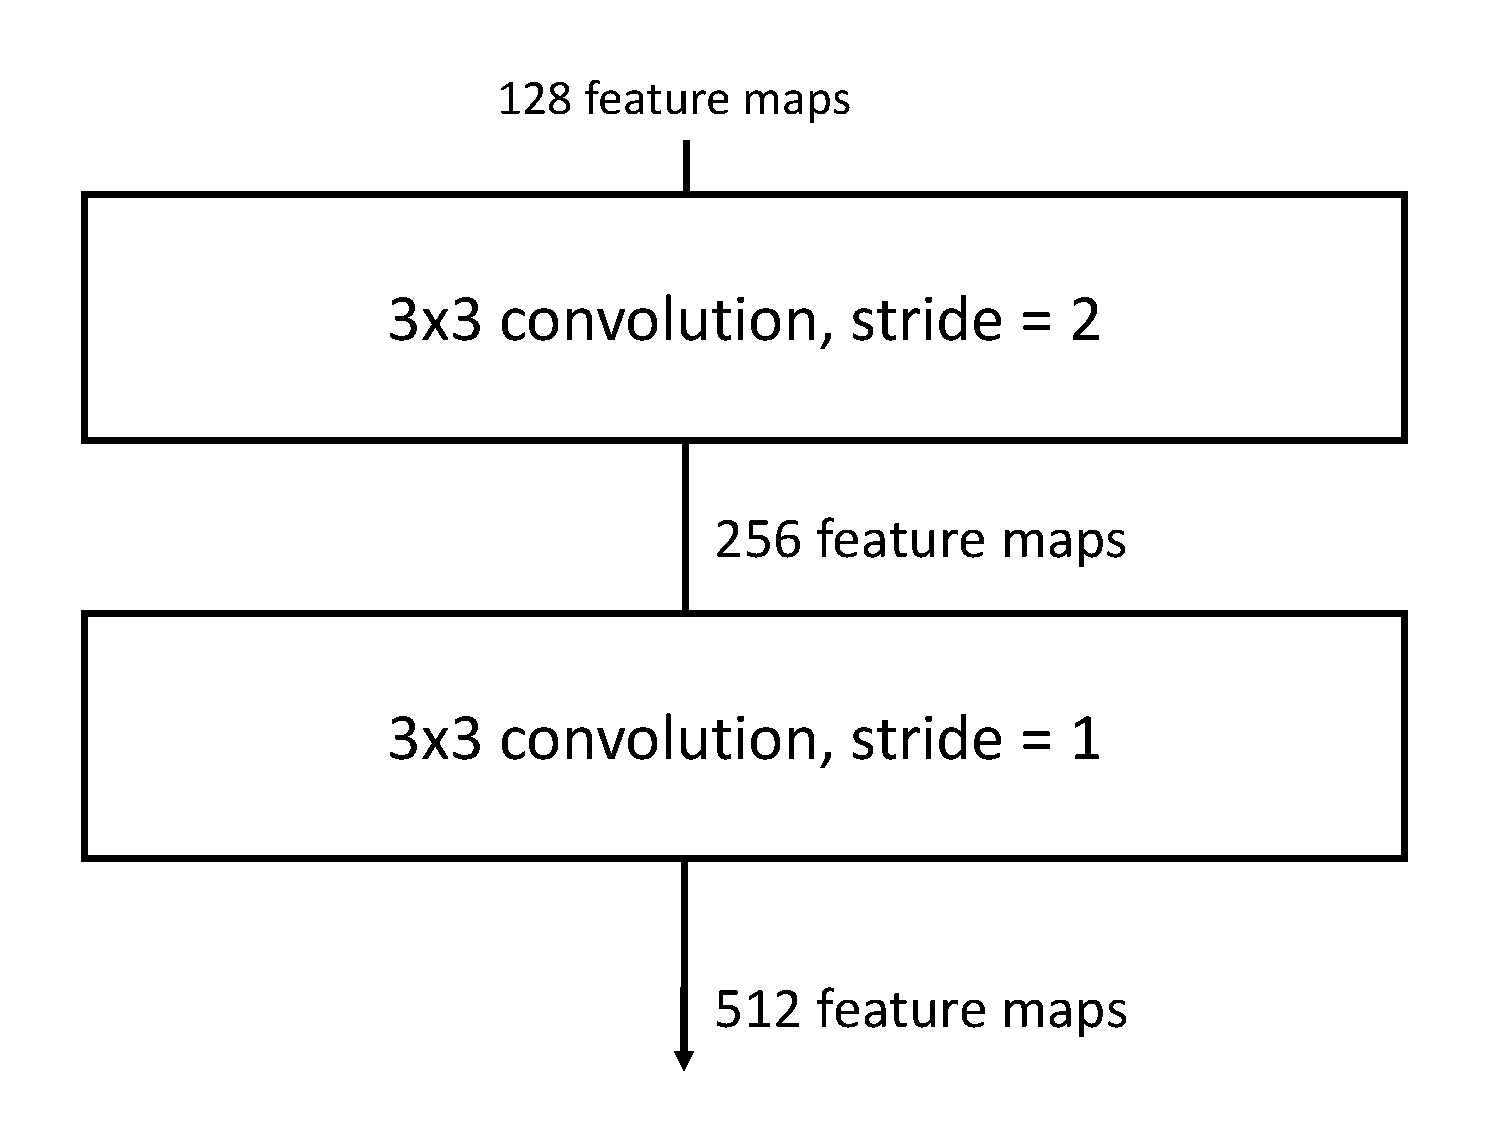
\includegraphics[width=0.45\textwidth]{FIG/cnnblock.pdf}
    \end{center}
    Given the input feature maps $\boldsymbol X \in
    \mathbb{R}^{64\times 64 \times 128}$, all convolutional
    layers perform zero-padding of $1$ on each side of $H$ and
    $W$ dimensions.
    \begin{enumerate}
    \item (5 points) What is the total number of parameters in
    the block (you can skip bias terms)?


    \item (5 points) What is the total number of multi-add
    operations in the block?


    \item (5 points) What is memory requirement change to store
    the input and output features of this block (Use percentage)?
    \end{enumerate}

    \item (45 points) \textbf{Neural Network for Image
    Recognition:} In this coding assignment, you will need to
    complete the implementation of a neural network
    (Fully-Connected Network for 474 students and Convolutional
    Neural Network for 574 students) using PyTorch and apply the
    network to the image recognition task on Cifar-10 (10-classes
    classification). You will need to install the python packages
    ``tqdm'' and ``pytorch''. Please read the installation guides
    of PyTorch here (https://pytorch.org/get-started/locally/).
    You are expected to implement your solution based on the
    given codes. The only file you need to modify is the
    ``solution.py'' file. You can test your solution by running
    the ``main.py'' file.
    
    \begin{enumerate}
    \item (25 points) Complete the class \emph{\textbf{Net()}}.
    In particular, define operations in function
    \emph{\textbf{\_\_init\_\_()}} and use them in function
    \emph{\textbf{forward()}}. The input of
    \emph{\textbf{forward()}} is an image.
    
    {\color{red} For 474 Students:} Please use
    \emph{\textbf{ReLU}} function to activate the outputs of the
    first two fully-connected layers. The sequential layers are:
    \begin{align*}
    &\text{Inputs} \to \\
    &\text{Reshape to vector}\to \text{Fully-connected (512 out units)}\to \\
    &\text{Fully-connected (512 out units)}\to \text{Fully-connected (n\_classes out units)}
    \end{align*}

    {\color{red} For 574 Students:}
    The sub-sampling is implemented by using the max pooling. And
    the kernel size for all the convolutional layers are $5\times
    5$. Please use \emph{\textbf{ReLU}} function to activate the
    outputs of convolutional layers and the first two
    fully-connected layers. The sequential layers of the network are:
    \begin{align*}
    &\text{Inputs} \to \\
    &\text{Convolution (6 out channels)} \to \text{Max Pooling} \to \\
    &\text{Convolution (16 out channels)}\to \text{Max Pooling}\to\\
    &\text{Reshape to vector}\to \text{Fully-connected (120 out units)}\to \\
    &\text{Fully-connected (84 out units)}\to \text{Fully-connected (n\_classes out units)}
    \end{align*}
    
    For this part, you are only allowed to use the APIs in
    \emph{\textbf{torch.nn}}. Please refer to the PyTorch API
    documents below for the usage of those APIs before you use
    them: \\
    https://pytorch.org/docs/stable/nn.html.

    Run the model by ``\emph{\textbf{python main.py}}'' and
    report the testing performance as well as a short analysis of
    the results.


    \item (10 points) Tune the hyperparameter of batch in ``\emph{\textbf{solution.py}}''. Please try 8, 16, 32, and 64. Run the model by
    ``\emph{\textbf{python main.py}}'' and report the testing
    performances as well as a short analysis of the results.


    \item (10 points) Tune the hyperparameter of learning rate (lr) in ``\emph{\textbf{solution.py}}''. Please try 0.01, 0.001, 0.0001, and 0.00001. 
    Run the model by ``\emph{\textbf{python main.py}}'' and
    report the testing performances as well as a short analysis of
    the results.

    
    \end{enumerate}
\end{enumerate}

\end{document}
